\begin{ParaColumn}[\section{Commands and Environments 命令与环境}]

    \switchcolumn[0]*[\subsection{Abstract Environment 摘要环境}]

    \verb"bilidoc" provides a bilingual abstract environment, its basic usage is:

    \switchcolumn

    \verb"bilidoc"提供了双语摘要环境,其基本用法为:

    \CrossColumnText{
        \begin{lstlisting}[language=LaTeX, caption=Abstract Environment, label=listing:abstract]
\begin{Abstract}{<English Key Words>}{<中文关键词>}[<Width of 1st Column>]
    <English Abstract>
    \switchcolumn
    <中文摘要>
\end{Abstract}
\end{lstlisting}
    }
    \switchcolumn*

    The parameters in curly brackets are required parameters, and the parameters in square brackets  are optional parameters.  \verb"<Width of 1st Column>" represents the width of the first column, that is, the width of the English abstract content. If this parameter is omitted, the first column width will take its default value \verb"0.60\linewidth".

    \switchcolumn

    花括号中的参数为必选参数,方括号中的参数为可选参数。\verb"<Width of 1st Column>"代表首列的宽度,即英文摘要内容的宽度,若省略该参数,则首列宽度取其默认值\verb"0.60\linewidth"。

    \switchcolumn*[\subsection{ParaColumn Environment 双栏环境}]

    The double-column environment \verb"ParaColumn" divides the page into two columns, and the contents of the two columns do not interfere with each other even when the document changes pages. This feature allows us to write bilingual translation documents.  The basic usage of \verb"ParaColumn" environment is:

    \switchcolumn

    双栏环境\verb"ParaColumn"将页面分为两栏,两栏的内容互不干扰,即使是在换页的情况下,这种特性允许我们编写双语对照翻译的文档。\verb"ParaColumn"环境的基本用法为:

    \CrossColumnText{
        \begin{lstlisting}[language=LaTeX, caption=ParaColumn Environment, label=listing:paracolumn]
\begin{ParaColumn}[<Width of 1st Column>]
    First Paragraph in English.
    \switchcolumn
    中文第一段。
    \switchcolumn*
    Second Paragraph in English.
    \switchcolumn
    中文第二段。
\end{Abstract}
\end{lstlisting}
    }
    \switchcolumn*
    
    Same as \verb"Abstract" environment, \verb"<Width of 1st Column>" represents the width of the first column, that is, the width of the English content. If this parameter is omitted, the first column width will take its default value \verb"0.60\linewidth".

    \switchcolumn

    与\verb"Abstract"环境相同的是,\verb"<Width of 1st Column>"代表首列的宽度,即英文内容的宽度,若省略该参数,则首列宽度取其默认值\verb"0.60\linewidth"。

    \switchcolumn*

    The difference between the command with a '*' \verb"\switchcolumn*" and \verb"\switchcolumn", is when we use \verb"\switchcolumn*" to switch from one column to another column, The content after the command will be aligned at the bottom of the content before the command, thus we can achieve the effect of aligning the top of each paragraph separately.

    \switchcolumn

    带‘*’号的命令~\verb"\switchcolumn*"~与命令\verb"\switchcolumn"不同的是,当我们使用\verb"\switchcolumn*"从一列切换到另一列时,该命令之后的内容将在该命令之前的内容的最底部对齐,即可实现每一小段顶部分别对齐的效果。

    \switchcolumn*

    The \verb"\switchcolumn*" command has an optional parameter before and after the'*' sign. The former can specify which column to switch to, and it is indicated by a number starting from 0. The latter can add a column text that spans two columns.  Generally, you can put commands such as \verb"\section" and \verb"\subsection" here to generate the title of the general column. You can also put the environment such as pictures and tables here, but you should put pictures and table codes in  Separate files, and then use the \verb"\input" command to import, otherwise unexpected results may occur.

    \switchcolumn

    \verb"\switchcolumn*"命令的'*'号的前后各有一个可选参数,前者可以指定具体切换到哪一列,用从0开始的数字表示,后者可以添加跨越两栏的通栏文本,一般可以将\verb"\section"和\verb"\subsection"等命令放到此处以产生通栏的标题,也可将图片和表格等环境放到此处,但你应该将图片和表格代码放到单独的文件,然后用\verb"\input"命令导入,否则可能会出现意想不到的结果。

    \CrossColumnText{
        \begin{lstlisting}[language=LaTeX]
\switchcolumn[0]*[\section{Getting Started 开始使用}]
\end{lstlisting}
    }
    
    \switchcolumn*

    The \verb"ParaColumn" environment may also start with a spanning text by specifying it as the optional argument of \verb"\begin{ParaColumn}".

    \switchcolumn

    \verb"ParaColumn"环境同样可以完成这种功能,只需在\verb"\begin{ParaColumn}"命令后添加相应的可选参数。

    \CrossColumnText{
        \begin{lstlisting}[language=LaTeX]
\begin{ParaColumn}[\section{Getting Started 开始使用}]
    ...
\end{ParaColumn}
\end{lstlisting}
    }

    \switchcolumn*[\subsection{CrossColumnText Command 跨栏命令}]

    As mentioned earlier, the \verb"\switchcolumn*" command can achieve the function of hurdling, but you cannot add equations here, otherwise an error will occur.  In order to add a hurdle equation, you can use the \verb"\CrossColumnText" command, which can also generate equation titles, tables and pictures.

    \switchcolumn

    前面提到,\verb"\switchcolumn*"命令可以实现跨栏的功能,但不能在此处添加公式,否则会产生错误。为了添加跨栏公式,可以使用\verb"\CrossColumnText"命令,该命令同样可以产生跨栏的标题、表格和图片等内容。

    \CrossColumnText{
        \begin{lstlisting}[language=LaTeX]
\CrossColumnText{
    \begin{align}
        ...
    \end{align}
}
\end{lstlisting}
    }

    \switchcolumn*[\subsection{BiliTable Environment 双语表格环境}]

    The bilingual table environment \verb"BiliTable" can generate a table with bilingual titles, see \enautoref{table:bilingual-table-example}, its basic usage is:
    
    \switchcolumn

    双语表格环境\verb"BiliTable"可以得到带双语标题的表格,见\cnautoref{table:bilingual-table-example}所示,其基本用法为:

    \CrossColumnText{
        \begin{lstlisting}[language=LaTeX, caption=Bilingual Table, label=listing:bilingual-table]
\begin{BiliTable}[<Options>]{<English Figure Name>}{<中文图名>}
    % <Table Content>
    \begin{tabular}[<Vertical Alignment>]{<Column Format>}
        ...
    \end{tabular}
\end{BiliTable}
\end{lstlisting}
        
\begin{lstlisting}[language=LaTeX, caption=Bilingual Table Example, label=listing:bilingual-table-example]
\begin{BiliTable}[!htb]{Properties of Skabo clay}{Skabo 黏土的物理特性}[table:bilingual-table-example]     
    \begin{tabular}{ll|ll}
        \Xhline{1pt}
        Properties & value & Properties & value \\
        \Xcline{1-4}{0.7pt}
        Water content, percent & 43.1 (39.4-47.8) & Activity & 0.63 \\
        Liquid limit & 52 & Salt content, g/L & 25 (24.2-28.8) \\
        Plastic limit & 24 & Organic content, percent & 0.32 \\
        Plastic index  & 28 & $S_u/p$ & 0.25 \\
        Clay fraction $<2\mu$, percent & 45 & Sensitivity & 5\\
        \Xhline{1pt}
    \end{tabular}
\end{BiliTable}
\end{lstlisting}

\begin{BiliTable}[float=!htb,label=table:bilingual-table-example]{Properties of Skabo clay}{Skabo 黏土的物理特性}
    \begin{tabular}{ll|ll}
        \Xhline{1pt}
        Properties & value & Properties & value \\
        \Xcline{1-4}{0.7pt}
        Water content, percent & 43.1 (39.4-47.8) & Activity & 0.63 \\
        Liquid limit & 52 & Salt content, g/L & 25 (24.2-28.8) \\
        Plastic limit & 24 & Organic content, percent & 0.32 \\
        Plastic index  & 28 & $S_u/p$ & 0.25 \\
        Clay fraction $<2\mu$ ,percent & 45 & Sensitivity & 5\\
        \Xhline{1pt}
    \end{tabular}
\end{BiliTable}
    }
    \switchcolumn*

    The optional parameter \verb"Options" controls the direction, hurdles, floating options and labels of the \verb"BiliTable" environment, different options are separated by commas. The following describes the options defined by the \verb"BiliTable" environment, The option on the right is its default value.

    \switchcolumn

    可选参数\verb"Options"控制\verb"BiliTable"环境的方向、跨栏、浮动选项以及标签,不同选项间用英文逗号隔开。下面描述了\verb"BiliTable"环境定义的选项,右侧选项为其默认值。

    \CrossColumnText{
        \vspace{3pt}
        \noindent
        \OptionsShow{orientation}{<vertical|horizontal|v|h>}{vertical}
        \vspace{3pt}
    }
    \switchcolumn*

    The \ColorCode{orientation} option is used to control the direction of the table. When the \ColorCode{orientation} option is \verb"horizontal", a single-page horizontal table will be generated.

    \switchcolumn

    \ColorCode{orientation}选项用于控制表格的方向,当\ColorCode{orientation}选项为\verb"horizontal"时,将生成单页的横向表格。

    \CrossColumnText{
        \vspace{3pt}
        \noindent
        \OptionsShow{crosscolumn}{<true|false>}{false}
        \vspace{3pt}
    }
    \switchcolumn*

    The \ColorCode{crosscolumn} option is used to generate a cross-column table, which is equivalent to the \verb"table*" environment.
    
    \switchcolumn

    \ColorCode{crosscolumn}选项用于产生跨栏表格,相当于\verb"table*"环境。

    \CrossColumnText{
        \vspace{3pt}
        \noindent
        \OptionsShow{label}{<name>}{}
        \vspace{3pt}
    }
    \switchcolumn*

    The \ColorCode{label} option is used to create label for the table, which is equivalent to defining \verb"\label{name}". You can use \verb"\ref{name}" to reference the table from other places.

    \switchcolumn

    \ColorCode{label}选项用于产生标签,相当于定义了\verb"\label{name}"命令,可从其它地方使用\verb"\ref{name}"引用该表格。

    \switchcolumn*

    The optional parameter \verb"FloatPlacement" is used to control the floating options of the float table, and its default value is \verb"htbp", the \verb"H" option provided by the \verb"float" package is used to create a non-floating table.

    \switchcolumn

    可选参数\verb"FloatPlacement"用于控制浮动体的浮动选项,其默认值为\verb"htbp",\verb"float"宏包提供的\verb"H"选项用于产生不浮动的表格。

    \CrossColumnText{
        \vspace{3pt}
        \noindent
        \OptionsShow{FloatPlacement}{[!]<\emph{subset of} htbp> \emph{or} <H>}{htbp}
        \vspace{3pt}
        \lstinputlisting[language=LaTeX, label=listing:bilingual-table-example]{tables/bilingual-table-example.tex}
    }
    \switchcolumn*

    The following \verb"listing" is an example of the \verb"BiliTable" environment, and the output result is shown in \enautoref{table:bilingual-table-example}.

    \switchcolumn

    下面的\verb"listing"是\verb"BiliTable"环境的一个示例,输出结果见\cnautoref{table:bilingual-table-example}所示。

    \switchcolumn*[\subsection{BiliFigure Environment 双语图形环境}]

    The bilingual figure environment \verb"BiliFigure" can generate a figure with bilingual titles, see \enautoref{figure:bilingual-figure-example}, its basic usage is:
    
    \switchcolumn

    双语图形环境\verb"BiliFigure"可以得到带双语标题的图形,如\cnautoref{figure:bilingual-figure-example}所示,其基本用法为:

    \CrossColumnText{
        \begin{lstlisting}[language=LaTeX, label=listing:bilingual-figure]
\begin{BiliFigure}[<Options>][<FloatPlacement>]{<English Figure Name>}{<中文图名>}
    % <Figure Content>
    \includegraphics[<Options>]{<Figure File Name>}
\end{BiliFigure}
\end{lstlisting}
        \begin{BiliFigure}[crosscolumn=true,label=figure:bilingual-figure-example][htb]{(a) Plasticity chart; (b) CPTU soil classification chart}{(a)可塑性图;(b)CPTU土壤分类图}     
    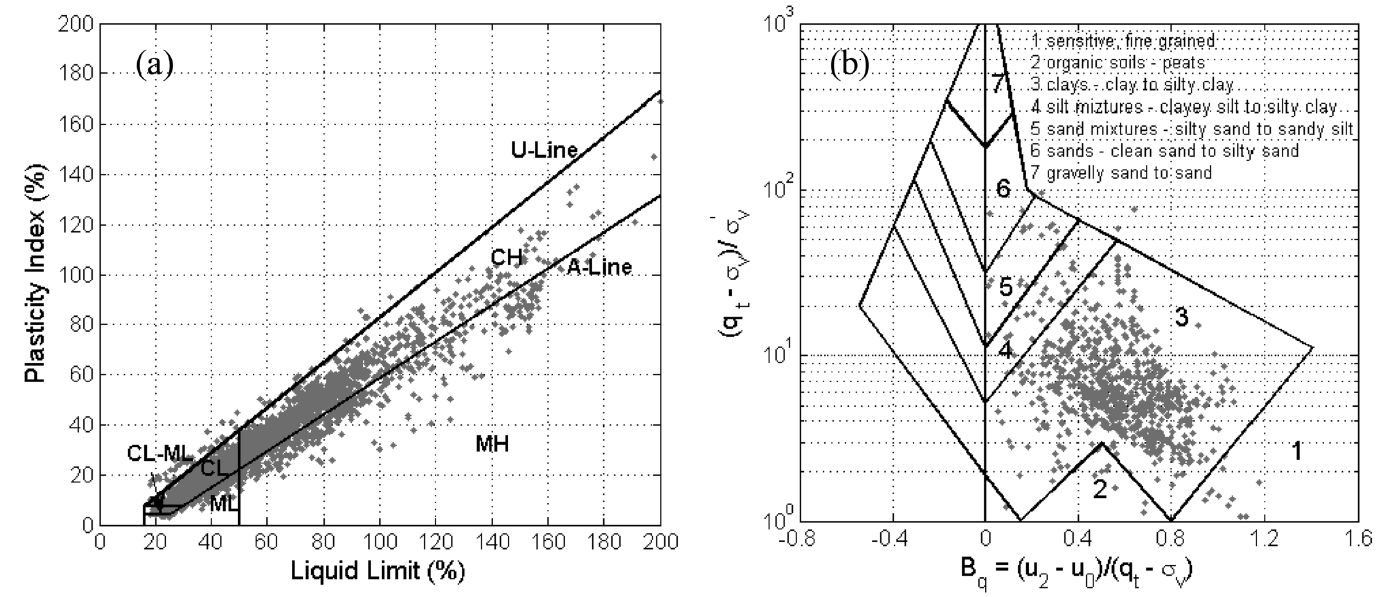
\includegraphics[width=0.80\linewidth]{figures/figure-1.png}
\end{BiliFigure}
    }
    \switchcolumn*

    The usage of the optional parameters of the bilingual picture  \verb"BiliFigure" environment \verb"Options" and the \verb"BiliTable" environment are basically the same, so I won't repeat them here.

    \switchcolumn

    双语图片\verb"BiliFigure"环境的可选参数\verb"Options"与\verb"BiliTable"环境的用法基本相同,这里不再赘述。

    \switchcolumn*

    The following \verb"listing" is an example of the \verb"BiliFigure" environment, and the output result is shown in \enautoref{figure:bilingual-figure-example}.

    \switchcolumn

    下面的\verb"listing"是\verb"BiliFigure"环境的一个示例,输出结果见\cnautoref{figure:bilingual-figure-example}所示。

    \CrossColumnText{
        \lstinputlisting[language=LaTeX, label=listing:bilingual-figure-example]{figures/bilingual-figure-example.tex}
    }
    \switchcolumn*

    In addition to inserting a single picture like \enautoref{figure:bilingual-figure-example}, we can also use the \verb"\subfigure" command provided by the \verb"subfigure" package to insert side-by-side subfigures, see \enautoref{figure:bilingual-subfigure-example}, its basic usage is:

    \switchcolumn

    除了像\cnautoref{figure:bilingual-figure-example}那样插入单张图片,我们还可以使用\verb"subfigure"宏包的\verb"\subfigure"命令插入并排的子图,如\cnautoref{figure:bilingual-subfigure-example}所示,其基本用法为:

    \CrossColumnText{
        \begin{lstlisting}[language=LaTeX, label=listing:bilingual-subfigure]
\begin{BiliFigure}[<Options>][<FloatPlacement>]{<English Figure Name>}{<中文图名>}
    \subfigure[<Subfigure Name>]{
        \includegraphics[<Options>]{<Subfigure File Name>}
        \label{<Subfigure Label>}
    }
    \subfigure[<Subfigure Name>]{
        \includegraphics[<Options>]{<Subfigure File Name>}
        \label{<Subfigure Label>}
    }
\end{BiliFigure}
\end{lstlisting}
        \begin{BiliFigure}[label=figure:bilingual-subfigure-example][htb]{Hvorslev Parameters}{Hvorslev参数}     
    \subfigure[Kawasaki Clays I]{
        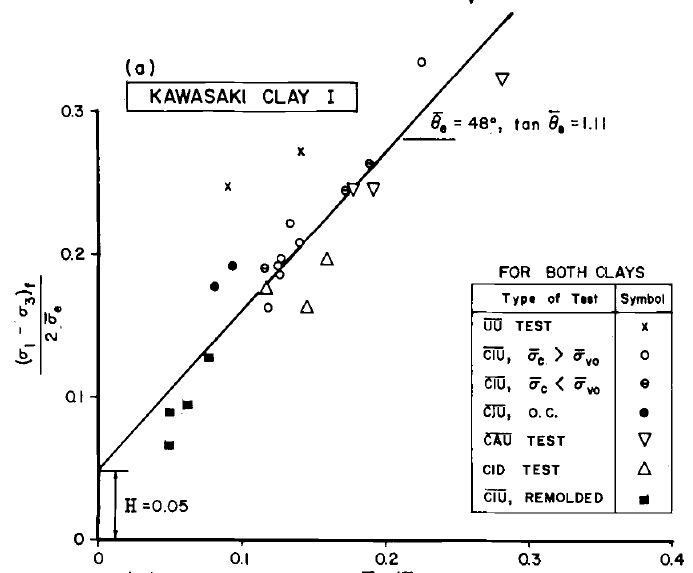
\includegraphics[width=0.36\textwidth]{figures/figure-2a.png}
        \label{figure:2a}
    }
    \subfigure[Lagunilla Clay]{
        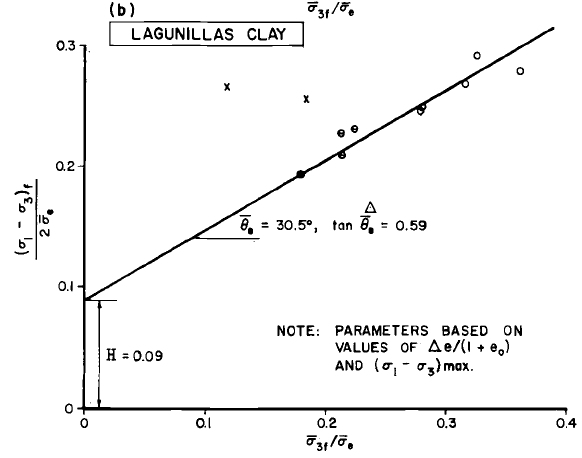
\includegraphics[width=0.36\textwidth]{figures/figure-2b.png}
        \label{figure:2b}
    }
\end{BiliFigure}
    }
    \switchcolumn*

    The following \verb"listing" is an example of \verb"subfigure", and the output result is shown in \enautoref{figure:bilingual-subfigure-example}.

    \switchcolumn
    
    下面的\verb"listing"是\verb"subfigure"的一个示例,输出结果见\cnautoref{figure:bilingual-subfigure-example}所示。

    \CrossColumnText{
        \lstinputlisting[language=LaTeX, label=listing:bilingual-subfigure-example]{figures/bilingual-subfigure-example.tex}
    }
    \switchcolumn*[\subsection{Side-by-Side Charts Command 图表横排命令}]

    The horizontal chart command \verb"\sidebyside" can typeset horizontal charts, see \enautoref{figure:side-by-side-charts-example-1} and \enautoref{figure:side-by-side-charts-example-2}, its basic usage is:

    \switchcolumn

    图表横排命令\verb"\sidebyside"可以排版横向并排的图表,如图\cnautoref{figure:side-by-side-charts-example-1}和\cnautoref{figure:side-by-side-charts-example-2}所示,其基本用法为:

    \CrossColumnText{
        \begin{lstlisting}[language=LaTeX, caption=Side-by-Side Charts Command, label=listing:side-by-side-charts]
\sidebyside[<Options>]
    {<Width of 1st Chart>}{<1st Chart Definition>}
    {<Width of 2nd Chart>}{<2nd Chart Definition>}
    [<Width of 3rd Chart>][<3rd Chart Definition>]
    [<Width of 4th Chart>][<4th Chart Definition>]
\end{lstlisting}
        \begin{lstlisting}[language=LaTeX, caption=Side-by-Side Charts Example, label=listing:side-by-side-charts-example]
\sidebyside[float=!htb]{0.50\linewidth}{
    \begin{BiliFigure}[float=H,label=figure:side-by-side-charts-example-1]{Relationship between $K_0$, $I_p$ and OCR}{$K_0$,$I_p$和OCR之间的关系}
        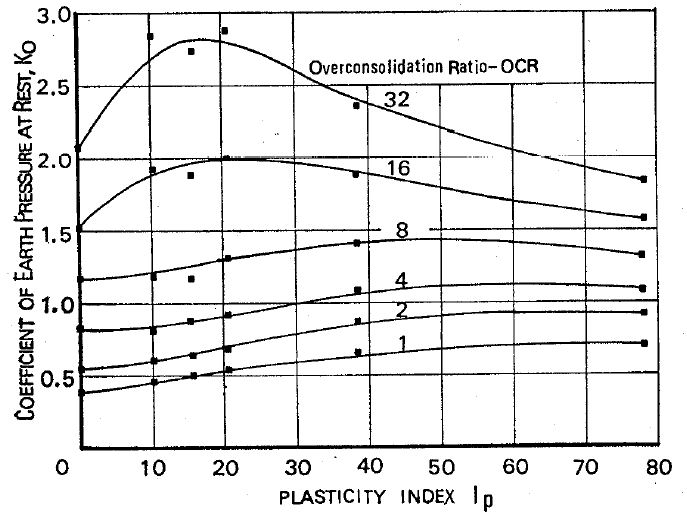
\includegraphics[width=\linewidth]{figures/figure-3}
    \end{BiliFigure}
}{0.45\linewidth}{
    \begin{BiliFigure}[float=H,label=figure:side-by-side-charts-example-2]{Trianguler classification chart}{三角分类图}
        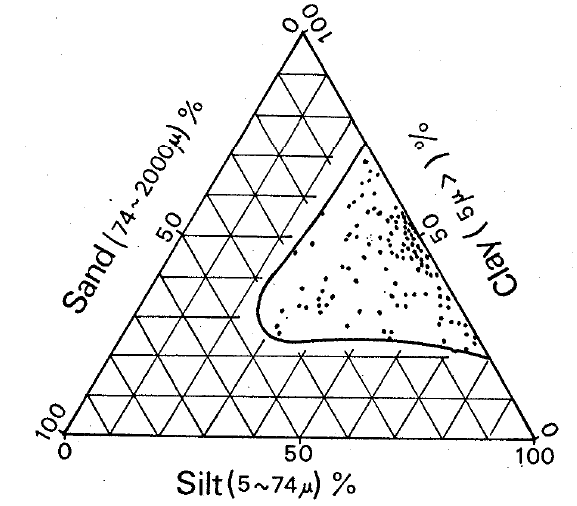
\includegraphics[width=\linewidth]{figures/figure-4}
    \end{BiliFigure}
}
\end{lstlisting}

\sidebyside[float=!htb]{0.50\linewidth}{
    \begin{BiliFigure}[float=H,label=figure:side-by-side-charts-example-1]{Relationship between $K_0$, $I_p$ and OCR}{$K_0$,$I_p$和OCR之间的关系}
        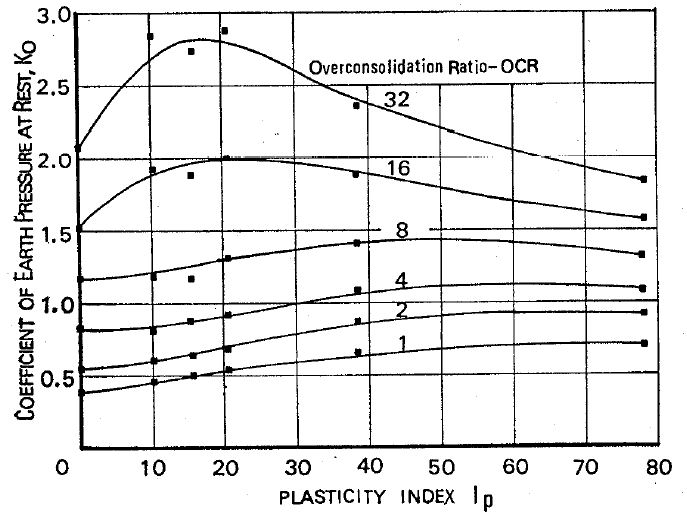
\includegraphics[width=\linewidth]{figures/figure-3}
    \end{BiliFigure}
}{0.45\linewidth}{
    \begin{BiliFigure}[float=H,label=figure:side-by-side-charts-example-2]{Trianguler classification chart}{三角分类图}
        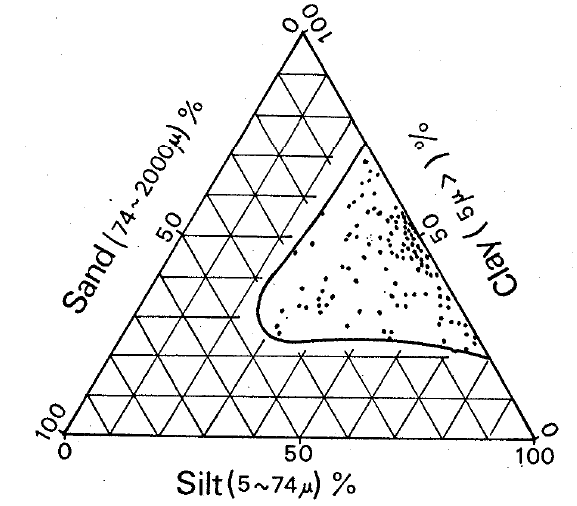
\includegraphics[width=\linewidth]{figures/figure-4}
    \end{BiliFigure}
}
    }
    \switchcolumn*

    The optional parameter \verb"Options" of the \verb"sidebyside" command provides \ColorCode{verticalalignment}, \ColorCode{crosscolumn} and \ColorCode{float} option.  The usage of \ColorCode{crosscolumn} and \ColorCode{float} option is the same as that of the \verb"BiliTable" and \verb"BiliFigure" environment.

    \switchcolumn

    \verb"\sidebyside"命令的可选参数\verb"Options"提供了\ColorCode{verticalalignment}、\ColorCode{crosscolumn}和\ColorCode{float}选项。\ColorCode{crosscolumn}以及\ColorCode{float}选项与\verb"BiliTable"和\verb"BiliFigure"环境对应选项的用法相同。

    \CrossColumnText{
        \vspace{3pt}
        \noindent
        \OptionsShow{verticalalignment}{<top|center|bottom|t|c|b>}{bottom}
        \vspace{3pt}
    }
    \switchcolumn*

    \ColorCode{verticalalignment} controls the vertical alignment of the horizontal chart.
    
    \switchcolumn

    \ColorCode{verticalalignment}控制横排图表的垂直对齐方式。

    \switchcolumn*

    The following \verb"listing" is an example of \verb"sidebyside" command, and the output result is shown in \enautoref{figure:side-by-side-charts-example-1} and \enautoref{figure:side-by-side-charts-example-2}.

    \switchcolumn

    下面的\verb"listing"是\verb"sidebyside"命令的一个示例,输出结果见\cnautoref{figure:side-by-side-charts-example-1}和\cnautoref{figure:side-by-side-charts-example-2}所示。

    \CrossColumnText{
        \lstinputlisting[language=LaTeX, label=listing:side-by-side-charts-example]{figures/side-by-side-charts-example.tex}
    }
    \switchcolumn*[\subsection{End-by-End Charts Command 图表竖排命令}]

    The vertical chart command \verb"\endbyend" can typeset vertical charts, see \enautoref{figure:end-by-end-charts-example-1} and \enautoref{figure:end-by-end-charts-example-2}, its basic usage is:

    \switchcolumn

    图表竖排命令\verb"\endbyend"可以排版竖向并排的图表,如\cnautoref{figure:end-by-end-charts-example-1}和\cnautoref{figure:end-by-end-charts-example-2}所示,其基本用法为:

    \CrossColumnText{
        \begin{lstlisting}[language=LaTeX, caption=End-by-End Charts Command, label=listing:end-by-end-charts]
\endbyend[<Options>]{<Width>}
    {<1st Chart Definition>}
    {<2nd Chart Definition>}
    [<3rd Chart Definition>]
    [<4th Chart Definition>]
\end{lstlisting}
        \endbyend[crosscolumn=false][htb]{\linewidth}{
    \begin{BiliFigure}[label=figure:end-by-end-charts-example-1][H]{An example of shear wave velocity measurement}{剪切波速度测量示例}
        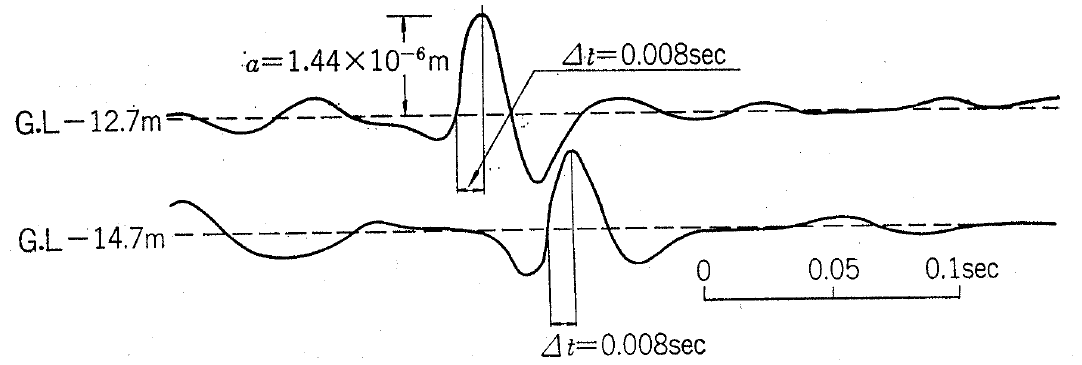
\includegraphics[width=0.3\linewidth]{figures/figure-5.png}
    \end{BiliFigure}
}{
    \begin{BiliFigure}[label=figure:end-by-end-charts-example-2][H]{Conceptual field loading condition}{概念性的场地加载条件}
        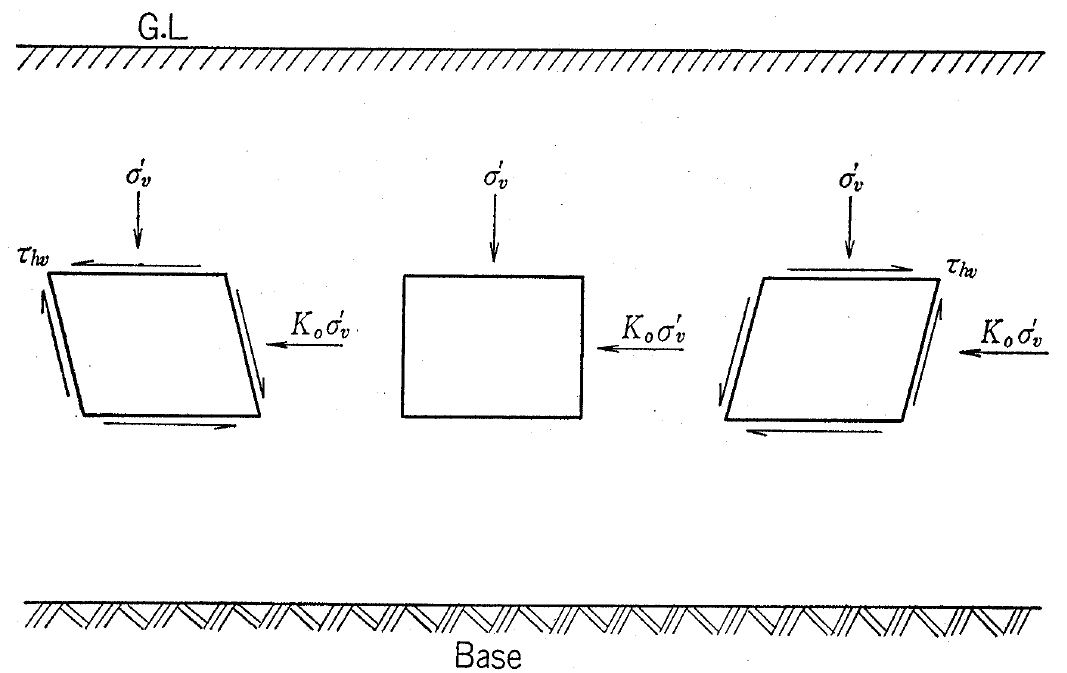
\includegraphics[width=0.3\linewidth]{figures/figure-6.png}
    \end{BiliFigure}
}
    }
    \switchcolumn*

    The optional parameter \verb"Options" of the \verb"sidebyside" command provides \ColorCode{crosscolumn} and \ColorCode{float} option.  Its usage is the same as that of the corresponding options of \verb"BiliTable" and \verb"BiliFigure". The parameter \verb"{<Width>}" is the width of the vertical chart environment.

    \switchcolumn

    \verb"\endbyend"命令的可选参数\verb"Options"提供了\ColorCode{crosscolumn}和\ColorCode{float}选项。它们的用法与\verb"BiliTable"和\verb"BiliFigure"环境对应选项的用法相同。参数\verb"{<Width>}"为整个竖排环境的宽度。

    \switchcolumn*

    The following \verb"listing" is an example of \verb"sidebyside" command, and the output result is shown in \enautoref{figure:end-by-end-charts-example-1} and \enautoref{figure:end-by-end-charts-example-2}.

    \switchcolumn

    下面的\verb"listing"是\verb"sidebyside"命令的一个示例,输出结果见\cnautoref{figure:end-by-end-charts-example-1}和\cnautoref{figure:end-by-end-charts-example-2}所示。

    \CrossColumnText{
        \lstinputlisting[language=LaTeX, label=listing:end-by-end-charts-example]{figures/end-by-end-charts-example.tex}
    }
    \switchcolumn*

    There is an interesting question worth discussing here.  Since we nested the \verb"BiliFigure" environment in the \verb"\endbyend" command, it involves the setting of two widths.  The \verb"\linewidth" in the outer \verb"\endbyend" command means that we have created a box with the width of \verb"\linewidth", and the content defined later will be typeset in this box, The horizontal alignment of the chart in the \verb"\endbyend"  command defaults to center alignment, so the final typesetting result is like \enautoref{figure:end-by-end-charts-example-1} and \enautoref{figure:end-by-end-charts-example-2} as shown.  If we change the width in the outer \verb"\endbyend" command to \verb"0.5\linewidth", then we will find that the final typesetting result will be centered in the left half.

    \switchcolumn

    这里有一个有趣的问题值得讨论。由于我们在\verb"\endbyend"命令中嵌套使用了\verb"BiliFigure"环境,于是涉及到了两个宽度的设置问题。外层\verb"\endbyend"命令中的\verb"\linewidth"表示我们创建了一个宽度为\verb"\linewidth"的盒子,之后定义的内容都将在这里盒子中进行排版,\verb"\endbyend"命令中图表的水平对齐方式默认为居中对齐,因此最终的排版结果如\cnautoref{figure:end-by-end-charts-example-1}和\cnautoref{figure:end-by-end-charts-example-2}所示。如果我们将外层\verb"\endbyend"命令中的宽度改为\verb"0.5\linewidth",这时我们会发现最终的排版结果将在左半区域居中对齐。

    \switchcolumn*
        
    Let's look at the width of the inner \verb"BiliFigure" environment again.  It is worth noting that the value of \verb"\linewidth" here is different from the name of \verb"\linewidth" of the outer \verb"\endbyend" command.  \verb"\linewidth" is actually the width of the environment where the command is located. For the outer \verb"\endbyend" command, \verb"\linewidth" is the width of the \verb"document" environment, which is the width of the heart of the document, and for the inner \verb"BiliFigure" environment, \verb"\linewidth" is the width of the box created by the \verb"\endbyend" command, which is the width value of the outer \verb"\endbyend" command.  If we change the width options of the outer \verb"\endbyend" command and the inner \verb"BiliFigure" environment to \verb"0.5\linewidth", then we will find the width of the picture finally created by the \verb"BiliFigure" environment becomes approximately \verb"0.25\linewidth".

    \switchcolumn

    我们再来看一下内层\verb"BiliFigure"环境中的宽度。值得注意的是,这里的\verb"\linewidth"在数值与外层\verb"\endbyend"命令的\verb"\linewidth"并不相同。\verb"\linewidth"为命令所处环境的宽度,对于外层\verb"\endbyend"命令,\verb"\linewidth"为\verb"document"环境的宽度,也就是文档版心的宽度,而对于内层\verb"BiliFigure"环境,\verb"\linewidth"为由\verb"\endbyend"命令创建的盒子的宽度,也就是外层\verb"\endbyend"命令的宽度值。如果我们将外层\verb"\endbyend"命令和内层\verb"BiliFigure"环境的宽度选项均改为\verb"0.5\linewidth",那么我们会发现最终由\verb"BiliFigure"环境创建的图片宽度变成了大约为\verb"0.25\linewidth"。

    \switchcolumn*[\subsection{Combination of Side-by-Side and End-by-End Charts 横排与竖排图表的组合}]

    If we need to typeset charts with more complicated position, such as one picture on the left and two pictures on the right, the \verb"\sidebyside" command and \verb"\endbyend" command obviously cannot satisfy us, at this time we can combine the two commands to achieve our purpose.

    \switchcolumn

    如果我们需要排版更复杂位置的图表,比如左侧排一张图,右侧以竖排的方式排两张图,\verb"\sidebyside"命令和\verb"\endbyend"命令显然都不能满足我们的需求,这时我们可以将两个命令结合起来以达到我们的目的。

    \switchcolumn*

    The following \verb"listing" is an example of the combination of \verb"sidebyside" and \verb"\endbyend" command, and the output result is shown in \enautoref{figure:combination-of-side-by-side-and-end-by-end-charts-example-1}$\sim$\enautoref{figure:combination-of-side-by-side-and-end-by-end-charts-example-3}.

    \switchcolumn
    
    下面的~\verb"listing"~是~\verb"\sidebyside"~命令和~\verb"\endbyend"~命令结合使用的一个示例,输出结果见\cnautoref{figure:combination-of-side-by-side-and-end-by-end-charts-example-1}$\sim$\cnautoref{figure:combination-of-side-by-side-and-end-by-end-charts-example-3}所示。

    \CrossColumnText{
        \lstinputlisting[language=LaTeX, label=listing:combination-of-side-by-side-and-end-by-end-charts-example]{figures/combination-of-side-by-side-and-end-by-end-charts.tex}
        \begin{lstlisting}[language=LaTeX, caption=Combination of Side-by-Side and End-by-End Charts Example, label=listing:combination-of-side-by-side-and-end-by-end-charts-example]
\sidebyside[float=!htb]{0.52\linewidth}{
    \begin{BiliFigure}[float=H,label=figure:combination-of-side-by-side-and-end-by-end-charts-example-1]{Perfect Sampling of a Normally Consolidated Clay and an Over-consolidated Clay}{正常固结土和超固结土的完美采样}
        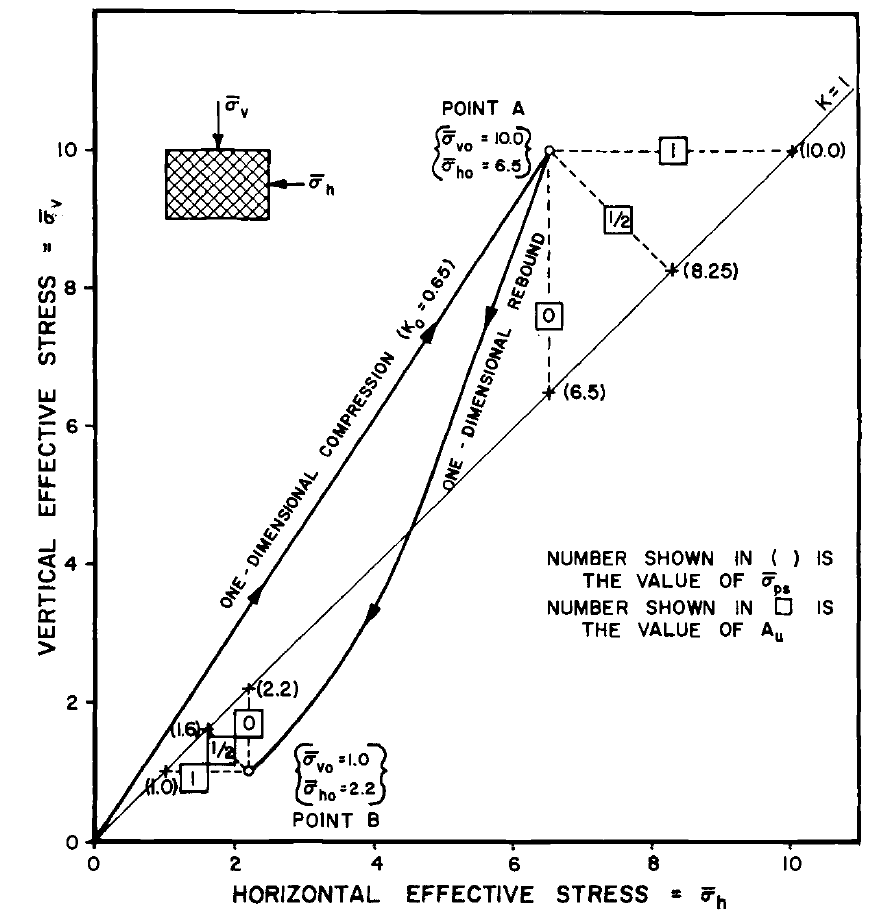
\includegraphics[width=\linewidth]{figures/figure-7.png}
    \end{BiliFigure}
}{0.44\linewidth}{
    \endbyend[float=H]{\linewidth}{
        \begin{BiliFigure}[float=H,label=figure:combination-of-side-by-side-and-end-by-end-charts-example-2]{An example of shear wave velocity measurement}{剪切波速度测量示例}
            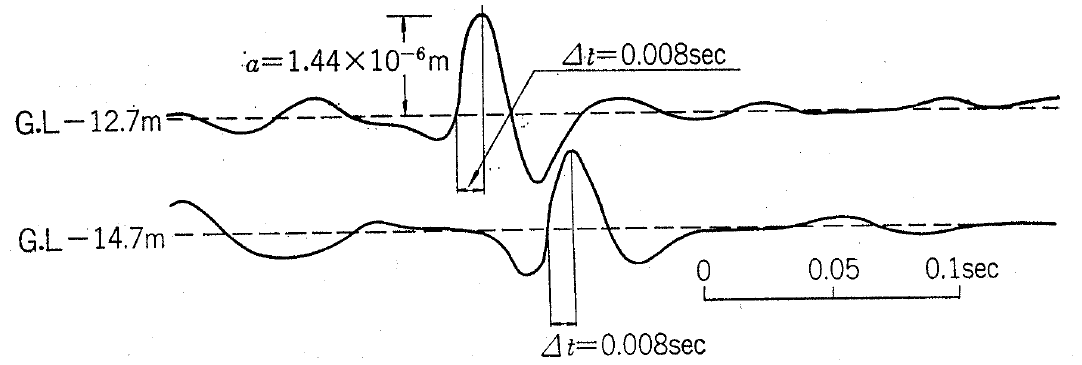
\includegraphics[width=\linewidth]{figures/figure-5.png}
        \end{BiliFigure}
    }{
        \begin{BiliFigure}[float=H,label=figure:combination-of-side-by-side-and-end-by-end-charts-example-3]{Conceptual field loading condition}{概念性的场地加载条件}
            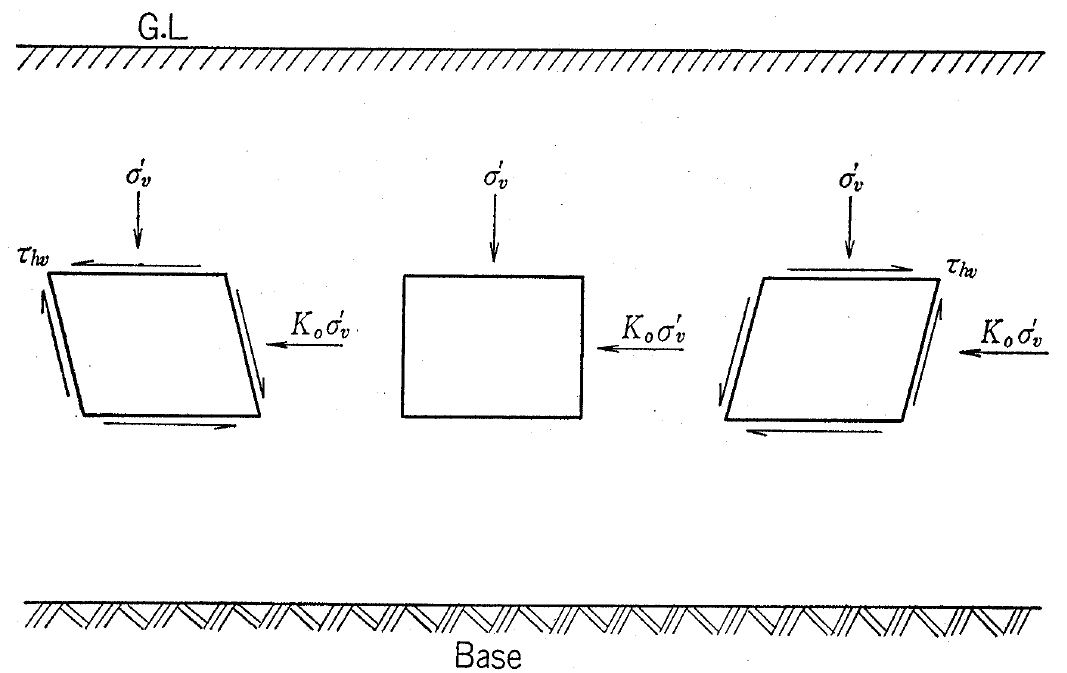
\includegraphics[width=\linewidth]{figures/figure-6.png}
        \end{BiliFigure}
    }
}
\end{lstlisting}

\sidebyside[float=!htb]{0.52\linewidth}{
    \begin{BiliFigure}[float=H,label=figure:combination-of-side-by-side-and-end-by-end-charts-example-1]{Perfect Sampling of a Normally Consolidated Clay and an Over-consolidated Clay}{正常固结土和超固结土的完美采样}
        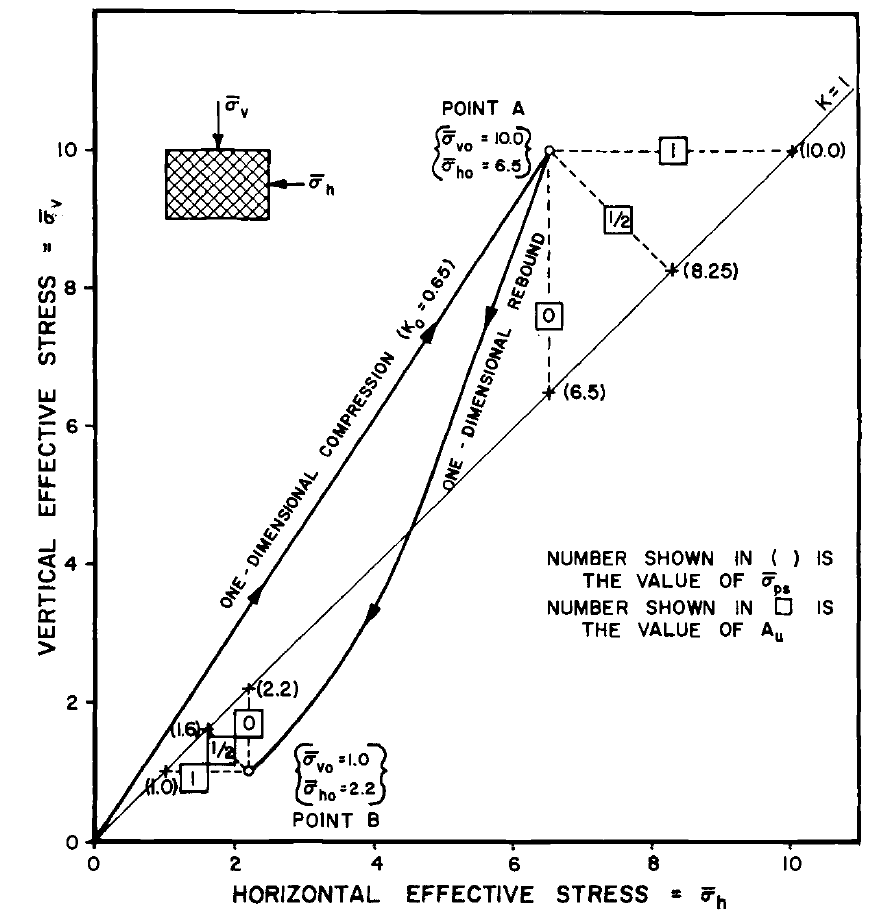
\includegraphics[width=\linewidth]{figures/figure-7.png}
    \end{BiliFigure}
}{0.44\linewidth}{
    \endbyend[float=H]{\linewidth}{
        \begin{BiliFigure}[float=H,label=figure:combination-of-side-by-side-and-end-by-end-charts-example-2]{An example of shear wave velocity measurement}{剪切波速度测量示例}
            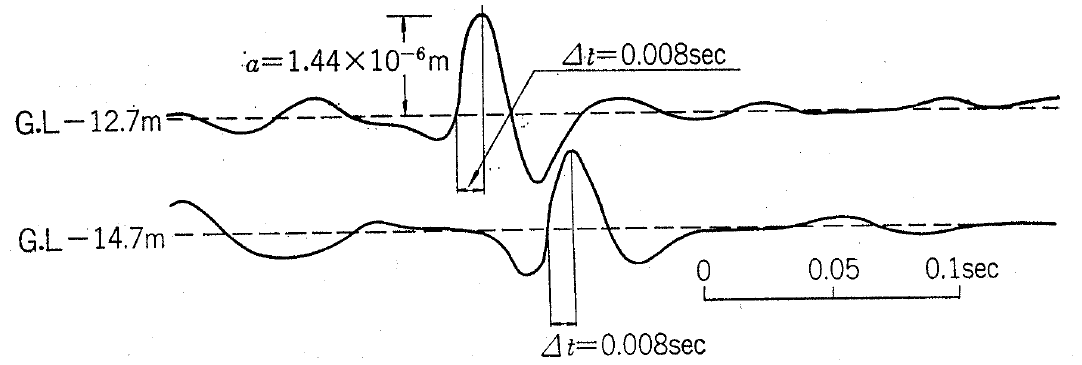
\includegraphics[width=\linewidth]{figures/figure-5.png}
        \end{BiliFigure}
    }{
        \begin{BiliFigure}[float=H,label=figure:combination-of-side-by-side-and-end-by-end-charts-example-3]{Conceptual field loading condition}{概念性的场地加载条件}
            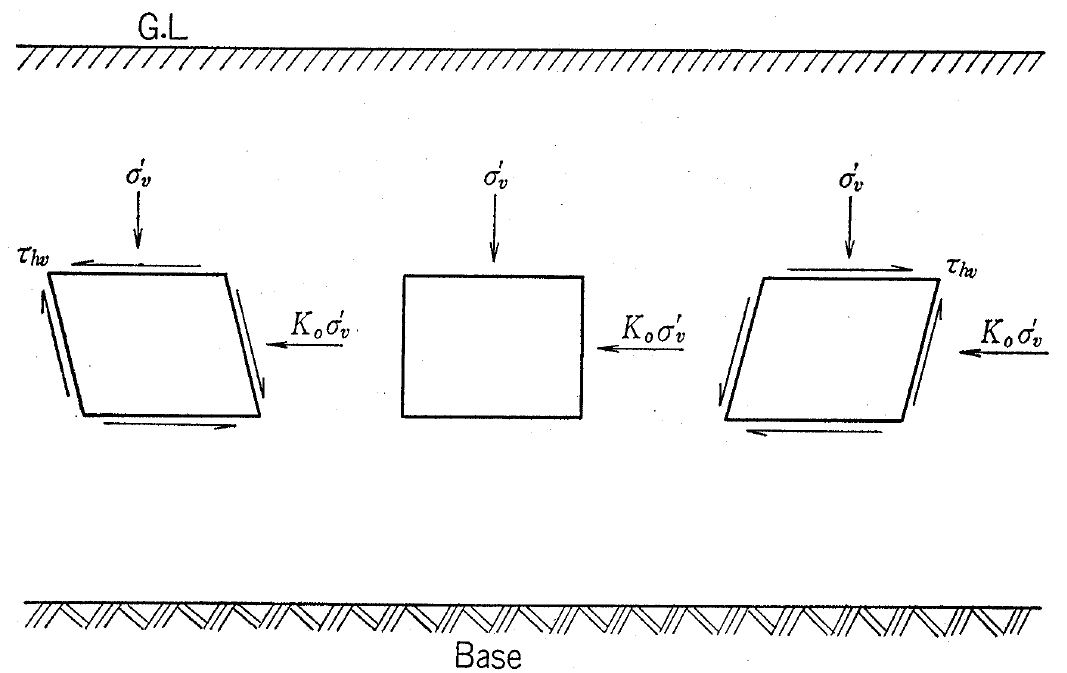
\includegraphics[width=\linewidth]{figures/figure-6.png}
        \end{BiliFigure}
    }
}

    }
    \switchcolumn*

    Here we will discuss the \verb"float" parameter of the above command again.  since the \verb"\sidebyside" and \verb"\endbyend" commands are based on the paragraph box \verb"minipage" environment, floating environments cannot be created in the box, the \verb"float" The parameter can only be set to the \verb"H" option provided by the \verb"float" package.  

    \switchcolumn

    这里我们再来讨论上述命令的\verb"float"参数。由于\verb"\sidebyside"和\verb"\endbyend"命令基于段落盒子\verb"minipage"环境, 盒子中不能创建浮动环境,因此该命令中图表定义中的\verb"float"参数只能设置为\verb"float"宏包提供的\verb"H"选项。

    \switchcolumn*
    
    For the above case, due to the nesting problem of the \verb"\sidebyside" and \verb"\endbyend" commands, only the \verb"float" parameter of the outer command can be set on your own, the \verb"float" parameter of the inner command can only be set to the \verb"H" option provided by the \verb"float" package.

    \switchcolumn
    
    对于上面所述的案列,由于涉及到了\verb"\sidebyside"和\verb"\endbyend"命令的嵌套问题,只有外层命令的\verb"float"参数可以自行设置,内层命令的\verb"float"参数都只能设置为\verb"float"宏包提供的\verb"H"选项。

    \switchcolumn*[\subsection{Cross Reference 交叉引用}]

    This document class has defined \verb"\cnautoref" and \verb"\enautoref" commands so that we can freely switch the cross-reference format in English and Chinese language environments.  \verb"\cnautoref" and \verb"\enautoref" commands accept \verb"label" from \verb"figure", \verb"subfigure", \verb"table", \verb"appendix" and \verb"equation", and automatically generate the corresponding application format, for example, \enautoref{figure:bilingual-figure-example}, \enautoref{figure:2a}, \enautoref{table:bilingual-table-example} et al.

    \switchcolumn

    本文档类定义了\verb"\cnautoref"命令以及\verb"\enautoref"命令,以便我们能在英文和中文两种语言环境中自由切换交叉引用的格式。\verb"\cnautoref"命令和\verb"\enautoref"命令接受来自\verb"figure"、\verb"subfigure"、\verb"table"、\verb"appendix"以及\verb"equation"的\verb"label",自动生成对应的应用格式,例如\cnautoref{figure:bilingual-figure-example}、\cnautoref{figure:2a}、\cnautoref{table:bilingual-table-example}等。

    \switchcolumn*[\subsection{Reference 参考文献}]

    For detailed usage of references, please refer to \href{https://www.ctan.org/pkg/natbib}{natbib} package or \href{https://www.ctan.org/pkg/gbt7714}{gbt7714} package.

    \switchcolumn

    参考文献的详细用法可参考\href{https://www.ctan.org/pkg/natbib}{natbib}宏包或\href{https://www.ctan.org/pkg/gbt7714}{gbt7714}宏包。

\end{ParaColumn}